\chapter{Evaluation}

In this chapter we will show some experiment results of our system. We will use various applications which will cover all the aspects of our implementation includes thread interleaving synchronization, application instrumentation and system call synchronization. With all the evaluation, we will answer the following questions:

\begin{itemize}
  \item Correctness: Given the same input, can the primary and secondary consistently generate the same output?
  \item Performance: Compare to non-replicated execution, how much overhead is introduced by our system?
  \item Breakdown: Where does the overhead come from?
\end{itemize}
% Evaluation factors:
% 1. Lock count & pcnmsg count for schedule part
% 2. Breakdown
% 3. Absolute time

\paragraph{Evaluation Setup} All experiments were run on a server machine with 4 AMD Opteron 6376 Processors (16 cores each, 2.3Ghz), which is 64 cores in total. The total RAM is 128GB. Our Popcorn Linux kernel was installed on Ubuntu 12.04 LTS. We partitioned the hardware resources into half, one for the primary and one for the secondary. Each of them has the full control of their own 32 cores and 64GB RAM. The machine comes with a 1Gbps high speed connection. For benchmarking server applications, we used a machine in the same rack, connected to the same switch, to act as the benchmark client.

\section{Racey}
We used a variant of racey~\cite{hillstress} to evaluate the correctness of our system. racey benchmark is a set of concurrent programs which read and write some shared data concurrently with various concurrent models. With a non-deterministic system, all the benchmark will create a different result during each different run. We use racey to validate if we can have the same thread interleaving on primary and secondary, which should lead the same output on both primary and secondary.

\paragraph{racey-guarded} racey-guarded has a global array, it uses pthread to create multiple threads and modify the global array concurrently. The access to the global array is protected by pthread\_mutex\_lock. We tested this one without any modification to the application. With both synchronization algorithms, we are able to create consistent results on the primary and secondary for over 100 consecutive runs.

\paragraph{racey-forkmmap} racey-forkmmap utilizes mmap to create a shared memory area, and uses fork to create multiple processes to read and modify the shared memory area. We manually added \_\_det\_start and \_\_det\_end around each access to the shared memory area. With both synchronization algorithms, we are able to create consistent results on the primary and secondary for over 100 consecutive runs.

\paragraph{racey-tcp} Based on the idea of racey, we developed racey-tcp to stress the determinism for I/O related tasks. racey-tcp uses pthread to create multiple threads. One thread listens to the socket, whenever a new connection arrives, it puts the connection into a queue, other threads retrieve the connection from the queue, read the data on that connection and write the data into a file. For this benchmark, we wrapped the write system call for writing to the file with \_\_det\_start and \_\_det\_end. With both synchronization algorithms, we are able to create consistent output file on the primary and secondary for over 2000 requests.

\section{PBZip2}
% 1. threading model
% 2. A table of lock and cond var count
% 3. A table of instrumented dettick count
PBZip2 is the parallel version of bzip2. The concurrent model of this application is a typical producer-consumer model, as shown in Figure~\ref{f:pbzip_model}. The FileReader thread reads the content of the file, break the input data into data chunks and put all the chunks into a queue. Worker threads get the data chunks from the queue and do the compression/decompression, after all put the produced data to another queue. The FileWriter will keep getting products from the queue and write them to the final zip file. Multiple pthread\_mutex\_lock and pthread\_cond\_wait functions are applied to provide the mutual exclusion to the access of the queues.

\begin{figure}
\centering
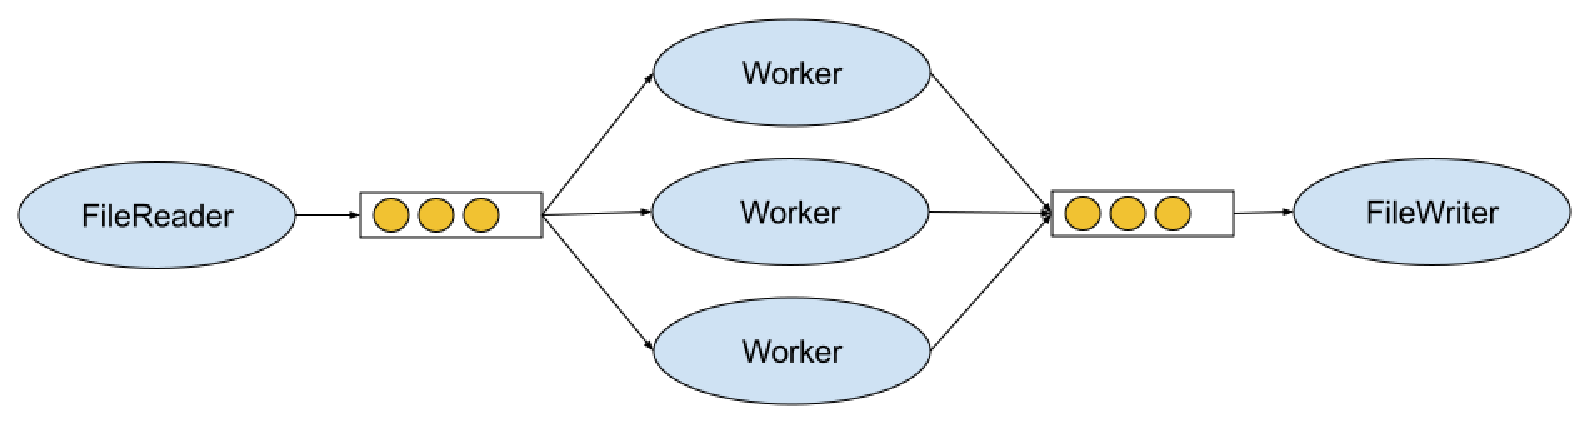
\includegraphics[width=0.8\columnwidth]{figures/pbzip2_model}
\caption{pbzip2 concurrent model}
\label{f:pbzip_model}
\end{figure}

For PBZip2, the time consuming part is the place where it calls the libz2 compression/decompression functions. In this benchmark, we utilized the execution time profiling instrumentation to balance the logical time for the deterministic execution, while for schedule replication nothing is modified. The benchmark is to compress a 177MB file with different thread counts, here we measure the performance with the total execution time reported by pbzip2.

Table~\ref{t:pbzip2_syscall} shows the system calls that are used by pbzip2, we only show the system calls that are tracked and synchronized by our system. In pbzip2,  gettimeofday is used for showing the time spent on the whole process, which it is not critical to the output of the application. However pthread\_cond\_timed\_wait also uses gettimeofday to calculate the timeout for the wait time, which is critical to the consistency of the execution.

\begin{table}
 \caption{Tracked system calls used by pbzip2}
\begin{center}
 \begin{tabular}{c | c}
 System Call & Use in the Application\\ \hline
 gettimeofday & Calculate execution time/pthread\_cond\_timed\_wait
 \end{tabular}
\end{center}
\label{t:pbzip2_syscall}
\end{table}

\paragraph{Correctness} For Deterministic Execution, any mismatch of the schedule will lead to different calling sequence of gettimeofday on the primary and secondary, which will result different reported execution time. For Schedule Replication, any mismatch of the schedule will lead the secondary waiting for a wrong schedule event forever. Neither of the case happened during the benchmark, the correctness of the replication thus proven.

\subsection{Results}

Figure~\ref{f:pbzip_b10_performance} shows the execution time of vanilla Linux, Deterministic Execution and Schedule Replication. Both replication modes achieved decent scalability. However, as we can see in Table~\ref{t:pbzip2_overall}, both algorithms' overhead increases with the thread count. One important overhead source for both replication modes comes from the serialization of all the synchronization primitives. With increasing thread count, the downside of breaking the parallelism of accessing those regions become more obvious.

For deterministic execution, another overhead comes from the calculation of the token. Current implementation requires O(N) time to decide which task should execute on next \detstart\ , where N is the number of threads. Every logical time update comes with such a computation process, more threads leads to more calculation time.

%different block sizes

\begin{table}
\caption{pbzip2 Overall Overhead of Each Replication Mode}
\begin{center}
 \begin{tabular}{c | c | c}
Thread count & Deterministic Execution & Schedule Replication \\ \hline
 2 & 14.27\% & 0.89\% \\ \hline
 4 & 22.89\% & 4.08\% \\ \hline
 8 & 33.82\% & 6.72\% \\ \hline
 16 & 69.00\% & 24.7\% \\ \hline
 24 & 100.02\% & 36.3\% \\ \hline 
 \end{tabular}
\end{center}
\label{t:pbzip2_overall}
\end{table}

\begin{figure}
\centering
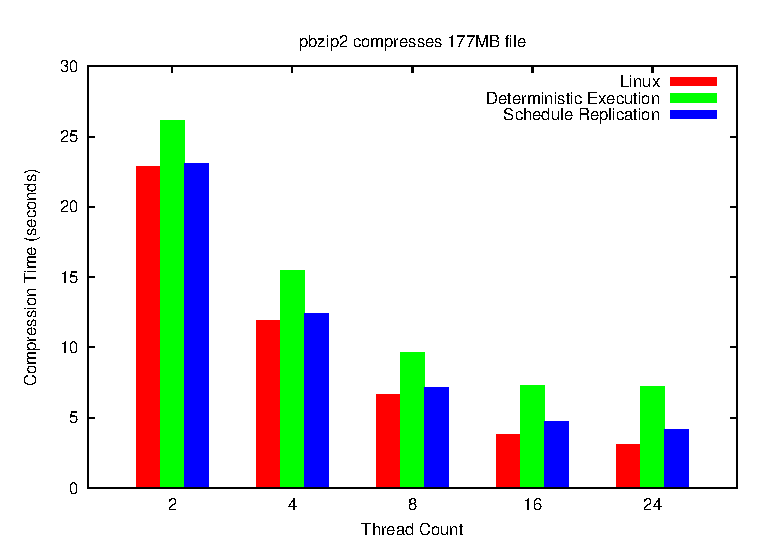
\includegraphics[width=0.8\columnwidth]{figures/pbzip2_b10}
\caption{pbzip2 performance}
\label{f:pbzip_b10_performance}
\end{figure}

\section{Mongoose Webserver}
% 1. threading model
% 2. A table of lock and cond var count

Mongoose is a compact multithreaded webserver. The concurrent model is shown in Figure~\ref{f:mongoose_model}. The MasterThread opens a listening socket, uses poll to wait for the incoming connections on the listening socket. Whenever a connection comes, the MasterThread accepts it and put the file descriptor to a queue. WorkerThreads get the connections from the queue and make the response to the clients. Table~\ref{t:mongoose_syscall} shows the system calls that are used by mongoose. The non-deterministic points in mongoose comes from both the thread-interleaving and system call output: diverged thread-interleaving leads to WorkerThreads handling incorrect sockets; diverged system call output leads to incorrect socket state and output value.

\begin{figure}
\centering
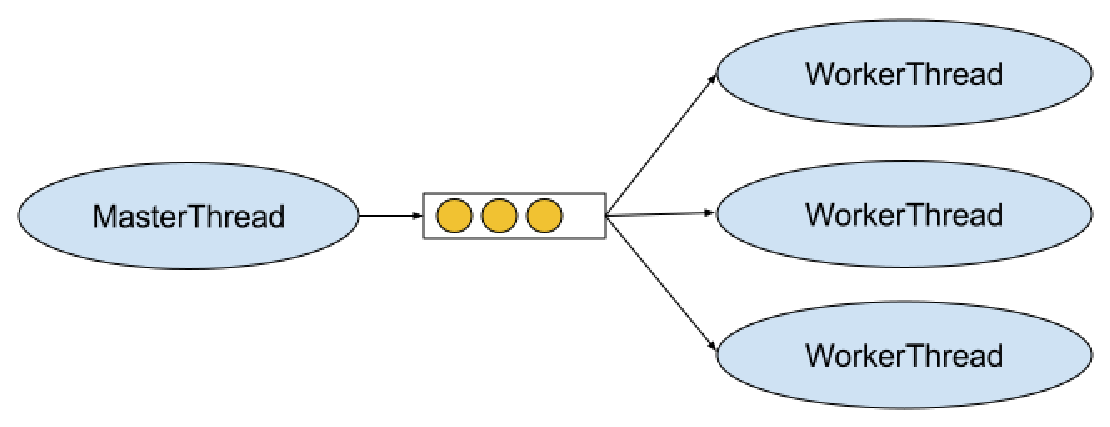
\includegraphics[width=0.6\columnwidth]{figures/mongoose_model}
\caption{mongoose concurrent model}
\label{f:mongoose_model}
\end{figure}

We used ApacheBench to stress test mongoose with different file sizes and different mongoose thread counts. Given mongoose's concurrent model, we can see that different file size will affect the frequency of acquiring locks. In this way we can figure out how will two algorithm perform under different lock acquisition load. Also, different thread counts can reflect the scalability of our system.
%cite ab

\begin{table}
\caption{Tracked system calls used by mongoose}
\begin{center}
 \begin{tabular}{c | c}
System Call & Use in the Application\\ \hline
 time & Generate HTTP header  \\ \hline
 poll & Wait for accept, read and write
 \end{tabular}
\end{center}
\label{t:mongoose_syscall}
\end{table}

\paragraph{Correctness} For both replication mode, any mismatch will lead to either different thread handling different socket, or divergence in the HTTP responses. Neither of the case happened during the benchmark, the correctness of the replication thus proven.

\subsection{Results}

\subsection{Overhead Breakdown}

\subsection{Message Breakdown}
In order to measure the message consumption of the benchmark, we put counters in different subsystems to count how many messages we need for each benchmark. Figure~\ref{f:mg_msg_4}, Figure~\ref{f:mg_msg_8} and Figure~\ref{f:mg_msg_16} show the breakdown of overall messages for each benchmark set. In all the figures, "Schedule Messages" means the messages for Tick Shepherd in Deterministic Execution, while in Schedule Replication this stands for the messages for logging the execution sequence.

% mongoose is using synchronous read and write

An interesting result is that actually we need much more messages for deterministic execution, which contradicts the assumption we made for Deterministic Execution. Bigger network payload leads to more socket calls, thus we need more messages for the Tick Shepherd to synchronize the tick bumps. However for Schedule Replication, since the messages for scheduling only depends on the number of synchronization primitives, which totally depends on the number of requests (not the size), as a result, across all the benchmarks, the number of schedule messages for Schedule Replication show a near constant value.

\begin{figure}
\centering
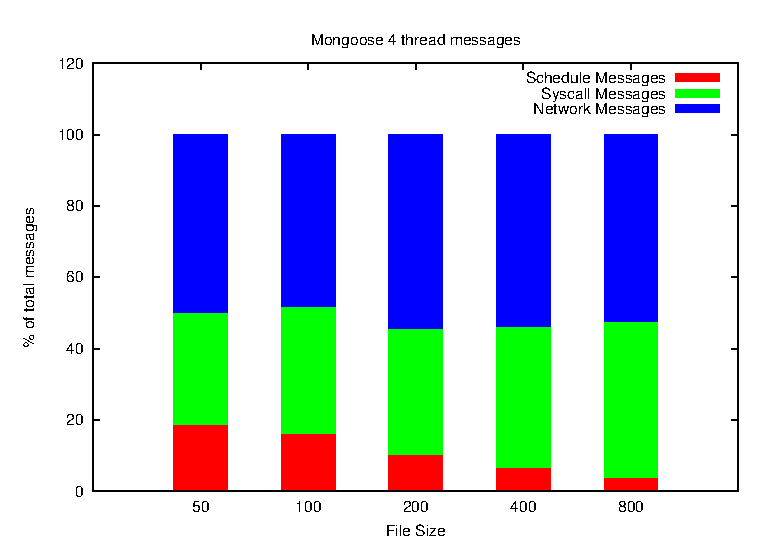
\includegraphics[width=1\columnwidth]{figures/mg_msg_4}
\caption{mongoose messages in 4 threads}
\label{f:mg_msg_4}
\end{figure}
\begin{figure}
\centering
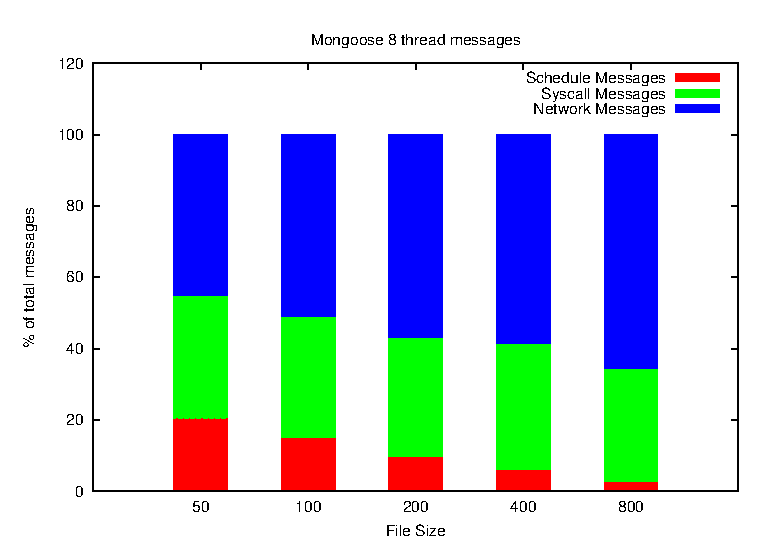
\includegraphics[width=1\columnwidth]{figures/mg_msg_8}
\caption{mongoose messages in 8 threads}
\label{f:mg_msg_8}
\end{figure}
\begin{figure}
\centering
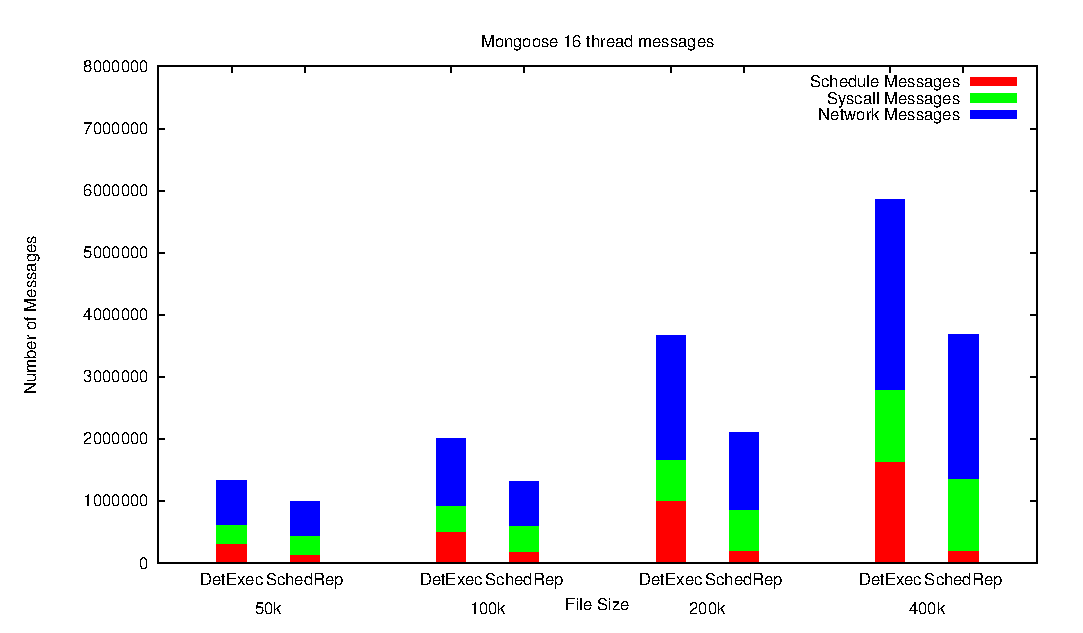
\includegraphics[width=1\columnwidth]{figures/mg_msg_16}
\caption{mongoose messages in 16 threads}
\label{f:mg_msg_16}
\end{figure}
\section{Nginx Webserver}
Nginx is a sophisticated webserver with multiple threading modes.

\begin{table}
\caption{Tracked system calls used by nginx}
\begin{center}
 \begin{tabular}{c | c }
System Call & Use in the Application\\ \hline
 time & Generate HTTP header\\ \hline
 epoll\_wait & Wait for accept, read and write
 \end{tabular}
\end{center}
\label{t:nginx_syscall}
\end{table}

\section{Redis Database Server}
Redis is an in-memory database server. It uses a single thread to process requests, but it dynamically creates new threads to write the in-memory data to the disk. This benchmark is perfect for stressing the flexibility of dealing with dynamically spawned threads.

For the performance test we used the redis-benchmark tool, we used the default benchmark parameter which will test all the operations. Each operation is tested for 10000 requests. We also have different number of concurrent clients to stress the server with different frequency of requests. We ran each setup for 5 times and took the average of the numbers.

Redis uses an alternative memory allocator jemalloc, which contains some internal locks to ensure mutual exclusion for concurrent memory allocation. As mentioned in Section~\ref{sec:elision}, those lock acquisitions doesn't affect the output at all, so we modified the jemalloc's source code, to skip the synchronizations for those locks.

\subsection{Results}
Figure~\ref{f:redis_2}, figure~\ref{f:redis_16} and figure~\ref{f:redis_64} show the  performance of redis with 2, 16 and 64 concurrent clients. Table~\ref{t:redis_overall} shows the overall overhead of each replication mode. 

\begin{figure}
\centering
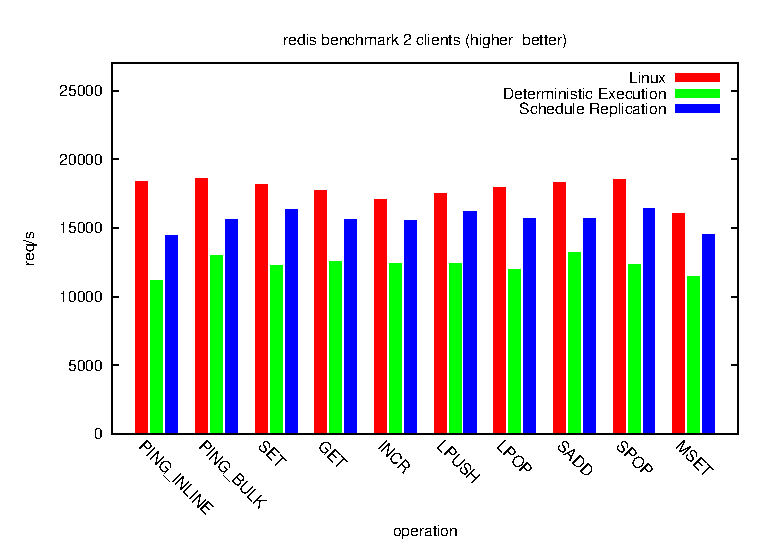
\includegraphics[width=0.8\columnwidth]{figures/redis_2}
\caption{redis benchmark with 10000 requests and 2 clients}
\label{f:redis_2}
\end{figure}

\begin{figure}
\centering
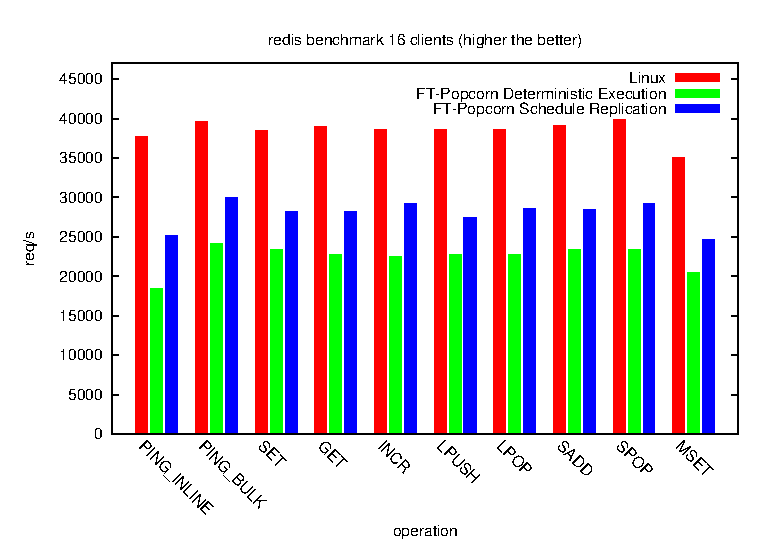
\includegraphics[width=0.8\columnwidth]{figures/redis_16}
\caption{redis benchmark with 10000 requests and 16 clients}
\label{f:redis_16}
\end{figure}

\begin{figure}
\centering
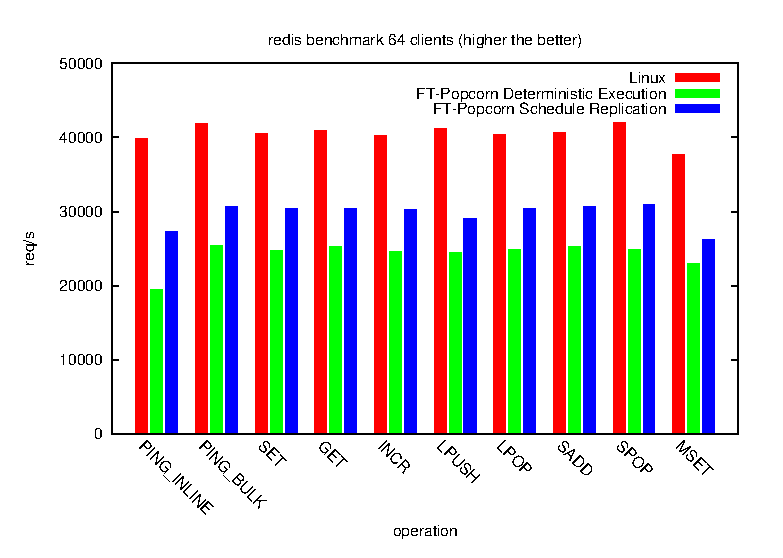
\includegraphics[width=0.8\columnwidth]{figures/redis_64}
\caption{redis benchmark with 10000 requests and 64 clients}
\label{f:redis_64}
\end{figure}

\begin{table}
\caption{Redis Overall Overhead of Each Replication Mode}
\begin{center}
 \begin{tabular}{c | c | c}
Client count & Deterministic Execution & Schedule Replication \\ \hline
 2 & 30.38\% & 11.93\% \\ \hline
 16 & 41.05\% & 26.94\% \\ \hline
 64 & 39.66\% & 26.48\% \\ \hline
 \end{tabular}
\end{center}
\label{t:redis_overall}
\end{table}

\subsection{Overhead Profiling}

\section{Discussion}
